%% Преамбула TeX-файла

% 1. Стиль и язык
\documentclass[utf8x, 14pt]{G7-32} % Стиль (по умолчанию будет 14pt)

% Остальные стандартные настройки убраны в preamble.inc.tex.
\sloppy

% Настройки стиля ГОСТ 7-32
% Для начала определяем, хотим мы или нет, чтобы рисунки и таблицы нумеровались в пределах раздела, или нам нужна сквозная нумерация.
\EqInChapter % формулы будут нумероваться в пределах раздела
\TableInChapter % таблицы будут нумероваться в пределах раздела
\PicInChapter % рисунки будут нумероваться в пределах раздела

% Добавляем гипертекстовое оглавление в PDF
\usepackage[
bookmarks=true, colorlinks=true, unicode=true,
urlcolor=black,linkcolor=black, anchorcolor=black,
citecolor=black, menucolor=black, filecolor=black,
]{hyperref}

\AfterHyperrefFix

\usepackage{microtype}% полезный пакет для микротипографии, увы под xelatex мало чего умеет, но под pdflatex хорошо улучшает читаемость

% Тире могут быть невидимы в Adobe Reader
\ifInvisibleDashes
\MakeDashesBold
\fi

\usepackage{graphicx}   % Пакет для включения рисунков

% С такими оно полями оно работает по-умолчанию:
% \RequirePackage[left=20mm,right=10mm,top=20mm,bottom=20mm,headsep=0pt,includefoot]{geometry}
% Если вас тошнит от поля в 10мм --- увеличивайте до 20-ти, ну и про переплёт не забывайте:
\geometry{right=20mm}
\geometry{left=30mm}
\geometry{bottom=20mm}
\geometry{ignorefoot}% считать от нижней границы текста


% Пакет Tikz
\usepackage{tikz}
\usetikzlibrary{arrows,positioning,shadows}

% Произвольная нумерация списков.
\usepackage{enumerate}

% ячейки в несколько строчек
\usepackage{multirow}

% itemize внутри tabular
\usepackage{paralist,array}

% Таблицы в альбомной ориентации
\usepackage{rotating}
\usepackage{lscape}
\usepackage{longtable}
\usepackage{multirow}

%\setlength{\parskip}{1ex plus0.5ex minus0.5ex} % разрыв между абзацами
\setlength{\parskip}{1ex} % разрыв между абзацами
\usepackage{blindtext}

% Центрирование подписей к плавающим окружениям
%\usepackage[justification=centering]{caption}

\usepackage{newfloat}
\DeclareFloatingEnvironment[
placement={!ht},
name=Equation
]{eqndescNoIndent}
\edef\fixEqndesc{\noexpand\setlength{\noexpand\parindent}{\the\parindent}\noexpand\setlength{\noexpand\parskip}{\the\parskip}}
\newenvironment{eqndesc}[1][!ht]{%
    \begin{eqndescNoIndent}[#1]%
\fixEqndesc%
}
{\end{eqndescNoIndent}}


%%% Вставка документов PDF в документ %%%
\usepackage[final]{pdfpages}


% Настройки листингов.
\ifPDFTeX
% 8 Листинги

\usepackage{minted}
%\usepackage{pygmentize}
\usepackage{listings}

% Значения по умолчанию
\lstset{
  basicstyle= \footnotesize,
  breakatwhitespace=true,% разрыв строк только на whitespacce
  breaklines=true,       % переносить длинные строки
%   captionpos=b,          % подписи снизу -- вроде не надо
  inputencoding=koi8-r,
  numbers=left,          % нумерация слева
  numberstyle=\footnotesize,
  showspaces=false,      % показывать пробелы подчеркиваниями -- идиотизм 70-х годов
  showstringspaces=false,
  showtabs=false,        % и табы тоже
  stepnumber=1,
  tabsize=4,              % кому нужны табы по 8 символов?
  frame=single
}

% Стиль для псевдокода: строчки обычно короткие, поэтому размер шрифта побольше
\lstdefinestyle{pseudocode}{
  basicstyle=\small,
  keywordstyle=\color{black}\bfseries\underbar,
  language=Pseudocode,
  numberstyle=\footnotesize,
  commentstyle=\footnotesize\it
}

% Стиль для обычного кода: маленький шрифт
\lstdefinestyle{realcode}{
  basicstyle=\scriptsize,
  numberstyle=\footnotesize
}

% Стиль для коротких кусков обычного кода: средний шрифт
\lstdefinestyle{simplecode}{
  basicstyle=\footnotesize,
  numberstyle=\footnotesize
}

% Стиль для BNF
\lstdefinestyle{grammar}{
  basicstyle=\footnotesize,
  numberstyle=\footnotesize,
  stringstyle=\bfseries\ttfamily,
  language=BNF
}

% Определим свой язык для написания псевдокодов на основе Python
\lstdefinelanguage[]{Pseudocode}[]{Python}{
  morekeywords={each,empty,wait,do},% ключевые слова добавлять сюда
  morecomment=[s]{\{}{\}},% комменты {а-ля Pascal} смотрятся нагляднее
  literate=% а сюда добавлять операторы, которые хотите отображать как мат. символы
    {->}{\ensuremath{$\rightarrow$}~}2%
    {<-}{\ensuremath{$\leftarrow$}~}2%
    {:=}{\ensuremath{$\leftarrow$}~}2%
    {<--}{\ensuremath{$\Longleftarrow$}~}2%
}[keywords,comments]

% Свой язык для задания грамматик в BNF
\lstdefinelanguage[]{BNF}[]{}{
  morekeywords={},
  morecomment=[s]{@}{@},
  morestring=[b]",%
  literate=%
    {->}{\ensuremath{$\rightarrow$}~}2%
    {*}{\ensuremath{$^*$}~}2%
    {+}{\ensuremath{$^+$}~}2%
    {|}{\ensuremath{$|$}~}2%
}[keywords,comments,strings]

% Подписи к листингам на русском языке.
\renewcommand\lstlistingname{Листинг}
\renewcommand\lstlistlistingname{Листинги}

\else
\usepackage{local-minted}
\fi

% Полезные макросы листингов.
\usepackage{listings}
% Любимые команды
\newcommand{\Code}[1]{\textbf{#1}}


\newcommand{\MainDomain}{digitaleconomy.space}
\newcommand{\MailDomain}{@digitaleconomy.space}
\newcommand{\CompanyName}{АНО "Цифровая Страна"}

%\usepackage[T2A]{fontenc}
%\usepackage{amssymb,amsfonts,amsmath,mathtext,cite,enumerate,float} %подключаем нужные пакеты расширений
%\def\labelitemi{--} %длинный минус для списоков
\graphicspath{{images/}}%путь к рисункам


\begin{document}
\begin{titlepage}
\newpage
\clearpage\maketitle
\thispagestyle{empty}

\begin{center}
\CompanyName \\
\vspace{0.1cm}
\hrulefill
\end{center}
 

\vspace{8em}

\begin{center}
\Large Руководство по работе с сайтами WordPress
\end{center}

\vspace{2.5em}
 
\begin{center}
\textsc{\textbf{Руководство администратора}}
\end{center}

\vspace{6em}
 

 
\vspace{\fill}

\begin{center}
Москва, \today
\end{center}

\end{titlepage}% это титульный лист
\tableofcontents % это оглавление, которое генерируется автоматически
\Introduction

В данном документе содержиться руководство по работе с сайтами WordPress (далее Система).\\

WordPress — система управления содержимым сайта с открытым исходным кодом (см. \url{https://ru.wordpress.org/} ).

\Abbreviations

В настоящем документе применяют следующие термины с соответствующими определениями:
\begin{description}
\item [API] (программный интерфейс приложения, интерфейс прикладного программирования) (англ. application programming interface, API) — набор готовых классов, процедур, функций, структур и констант, предоставляемых приложением (библиотекой, сервисом) или операционной системой для использования во внешних программных продуктах.
\item [JSON] (англ. JavaScript Object Notation) текстовый формат обмена данными.
\item [GUI] (англ. Graphical User Interface) графический пользовательский интерфейс.
\item [ТТ] (англ. Trouble Ticket) Зарегистрированное обращение о проблеме или инциденте.
\item [АС] автоматизированные системы.
\item [АРМ] автоматизированное рабочее место.
\item [БД] база данных.
\item [ВМ] виртуальная машина.
\item [ЗИП] Запасные части, инструменты, принадлежности
\item [ИР] информационные ресурсы.
\item [ИТ] информационные технологии.
\item [НСД] несанкционированный доступ.
\item [ПК] Персональный компьютер
\item [ПО] программное обеспечение.
\item [СЗИ] средства защиты информации.
\item [СУБД] Система управления базами данных.
\item [СХД] система хранения данных.
\item [Узел сети] это объект сети (физический, виртуальный), который необходимо наблюдать. Это может быть физический сервер, сетевой коммутатор, виртуальная машина или какое-нибудь приложение.

\end{description}% основное окно программы
\chapter{Панель Администратора}
\label{sec:chapter_admin}

В системе WordPress существует административная консоль системы управления сайтом, где вебмастер может добавлять или изменять контент своего блога, а также проводить различные изменения и усовершенствования по дизайну и функциям сайта.

Для входа в консоль администратора откройте страницу по адресу http://\MainDomain /wp-login.php (см. рис. \ref{fig:pic_Login})

\begin{figure}[htp]
    \centering
	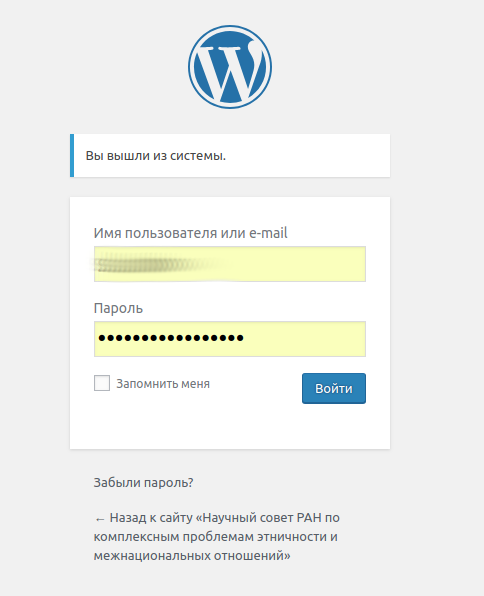
\includegraphics[width=0.3\textwidth]{login.png}
    \caption{Вход в Систему}
    \label{fig:pic_Login}
\end{figure}


После входа в систему откроется консоль администратора сайта (см. рис. \ref{fig:pic_welcome})

\begin{figure}[htp]
    \centering
	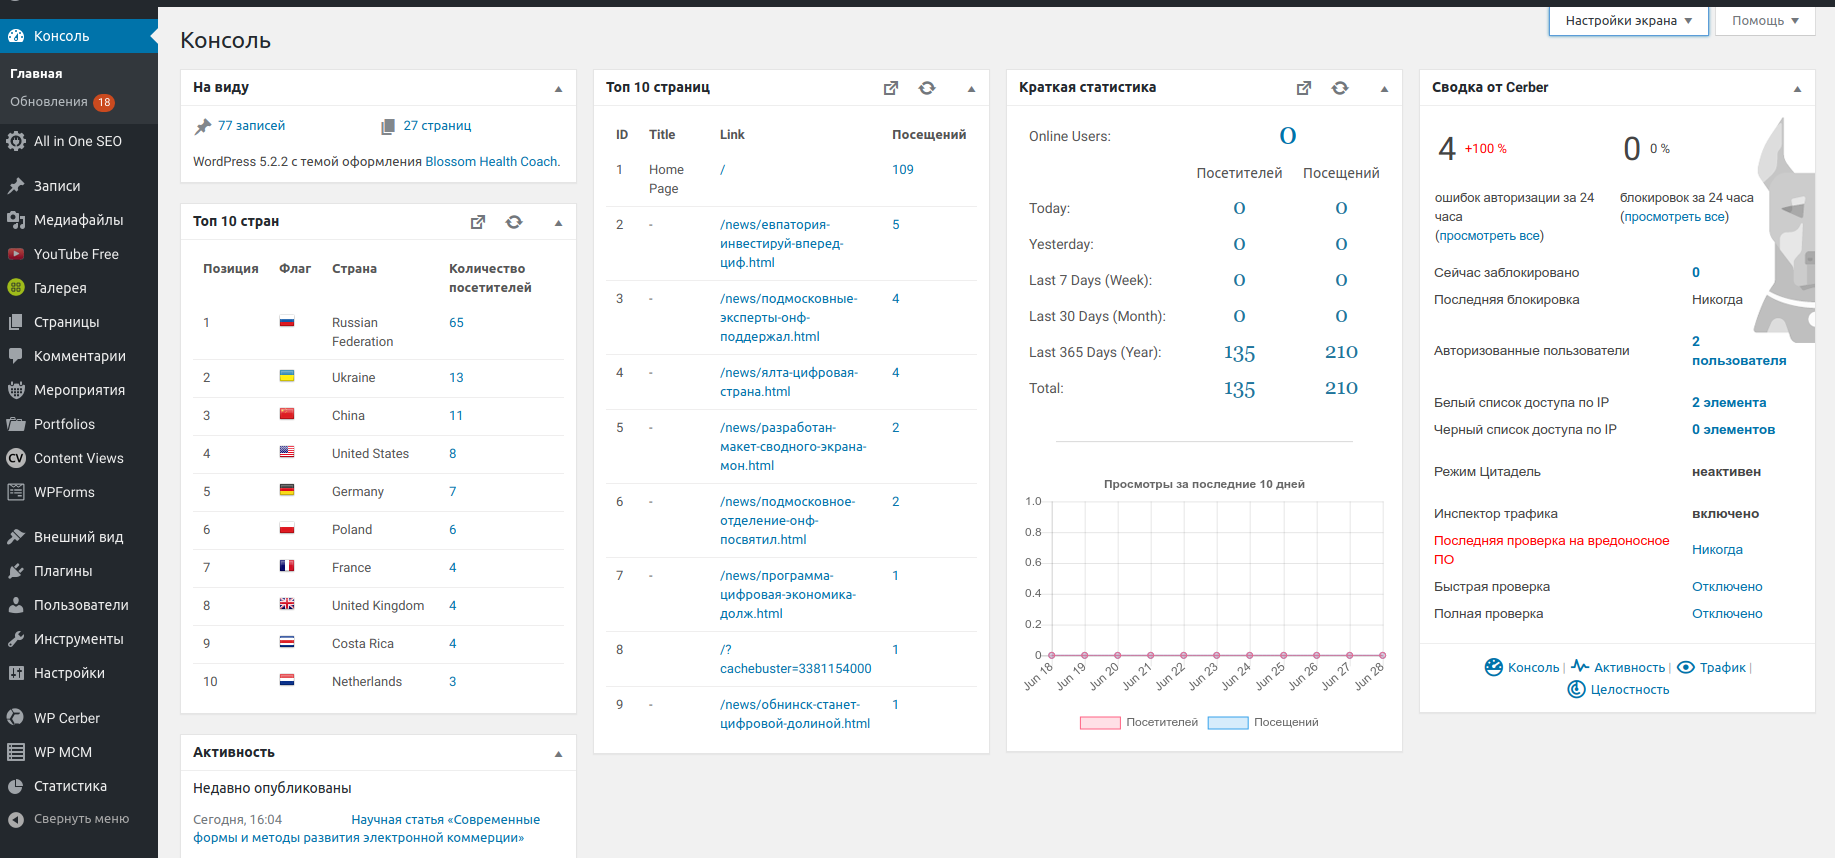
\includegraphics[width=\textwidth]{welcome.png}
    \caption{Стартовая страница администратора}
    \label{fig:pic_welcome}
\end{figure}

В правом верхнем углу есть кнопка «Настройки экрана». С ее помощью можно настроить все, что должно отображаться на странице.

Из перечисленного списка можно выбрать свежие комментарии, плагины, входящие ссылки, быструю публикацию, свежие черновики, блог, другие новости WordPress.

Слева на главной странице админки WordPress расположено вертикальное меню основных функций, которыми может воспользоваться вебмастер, его можно свернуть или развернуть.

К примеру, чтобы добавить запись, нужно перейти в раздел «Записи». В разделе «Внешний вид» устанавливается дизайн сайта, виджеты, меню, а также располагается редактор HTML. Не менее важны разделы «Плагины», «Инструменты» и «Параметры».

\section{Настройки}
\label{sec:part_wp_settings}

Настройки в админ панели WordPress, находятся в разделе «Параметры» — это самый важный раздел, в котором следует разобраться в первую очередь.

При нажатии на «Параметры» открывается выпадающее меню, которое содержит следующие группы настроек:

\begin{itemize}
\item Общие;
\item Написание;
\item Чтение;
\item Обсуждение;
\item Медиафайлы;
\item Постоянные ссылки.
\end{itemize}

\subsection{Общие настройки}
\label{sec:part_wp_settings_common}

В данном разделе вебмастер может задать название блога и его описание, которые будут находиться на основной странице сайта, а также использоваться в выдаче поисковых систем.
Следующий пункт в разделе «Общие» это адрес сайта и адрес WordPress. Рекомендуется указать одинаковый адрес, идентичный URL, чтобы в дальнейшем это не вызвало путаницы.

После этого в соответствующем поле вебмастер может указать свой действующий e-mail адрес, куда будут приходить все уведомления от WordPress, будь то свежие комментарии или обновленные настройки.

Затем следует очень интересный пункт под названием «Членство». Ставя под ним галочку, вебмастер разрешает регистрацию пользователей на своем ресурсе, но если смотреть объективно, данная функция бывает полезна владельцам блогов довольно редко.

В завершении общих настроек можно выбрать необходимый часовой пояс, формат даты и времени.

\subsection{Написание}
\label{sec:part_wp_settings_write}

В разделе «Написание» вебмастер может настроить отложенную публикацию и публикацию через e-mail адрес.
Здесь лучше оставить все как есть, потому, что большинству пользователей данная функция не пригодится.

\subsection{Чтение}
\label{sec:part_wp_settings_read}

В разделе «Чтение» владелец сайта может настроить страницу, которая будет главной. Это может быть статическая страница или последние записи на блоге. В роли статической главной страницы может выступать домашняя страница или любая другая, в том числе и специально созданная автором блога.
В данном разделе можно настроить, количество записей, которые будут отображаться на одной странице. А также настроить количество элементов, которые будут отображаться в RSS записях.

Последним пунктом в разделе является «Видимость для поисковых систем». Галочку здесь ставить не нужно, иначе сайт не будет проиндексирован.

\subsection{Обсуждение}
\label{sec:part_wp_settings_blog}

В разделе «Обсуждение» настраивается все, что так или иначе связано с комментариями. Это настройки по умолчанию, другие настройки комментариев, настройки отправления письма, модерация комментариев.
Медиафайлы

В разделе «Медиафайлы» владелец блога может задать необходимую ширину и высоту миниатюры изображений, а также максимальную ширину и высоту для изображений средних и крупных размеров.

\subsection{Постоянные ссылки}
\label{sec:part_wp_settings_links}

«Постоянные ссылки» — один из самых важных разделов админки wordpress. Здесь вебмастер имеет возможность настроить вид отображаемой ссылки, который больше всего для него подходит.

Ссылка может иметь название по умолчанию, может быть в виде даты и названия записи, месяца и названия записи, в виде цифр, названия или иметь произвольный формат.

Самым оптимальным вариантом является ссылка в виде одного названия. Так, владелец сайта может давать название ссылки идентичное названию статьи, только латинскими символами.

Это дает сайту огромное преимущество в поисковой выдаче, к тому же ссылки в виде названий статьи более приятны для посетителей сайта.

% 
\chapter{Медиафайлы}
\label{sec:chapter_media}

В библиотеку медиафайлов можно загружать изображения, звуковые файлы, видео и файлы других типов. Какие-то файлы публикуются для просмотра и прослушивания, а другие - для скачивания.
Для просмотра медиафайлов выберите меню «Медиафайлы/Библиотека» (см. рис. \ref{fig:pic_media_library})

\begin{figure}[htp]
    \centering
	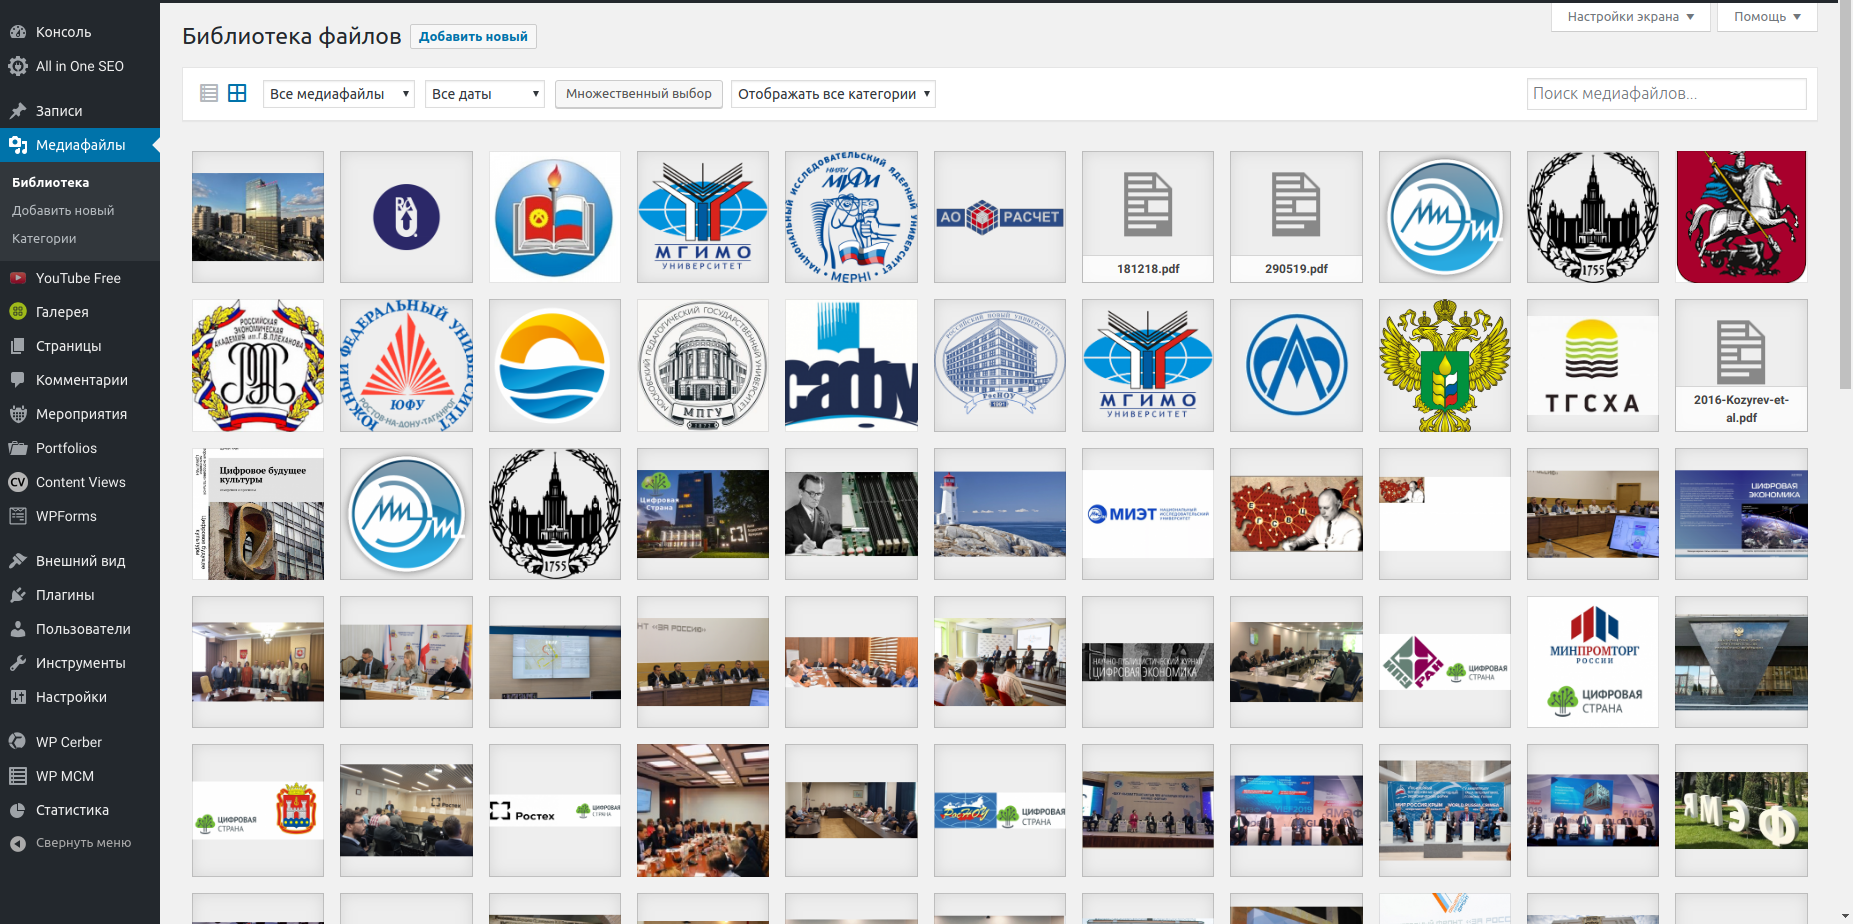
\includegraphics[width=\textwidth]{media_library.png}
    \caption{Библиотека медиафайлов}
    \label{fig:pic_media_library}
\end{figure}


\section{Категории медиафайлов}
\label{sec:part_cat_media}

Категории медиафайлов служат для удобства их поиска.
Создать или редактировать (удалить) категорию можно в разделе меню «Медиафайлы/Media Categories» (см. рис. \ref{fig:pic_media_library})

\begin{figure}[htp]
    \centering
	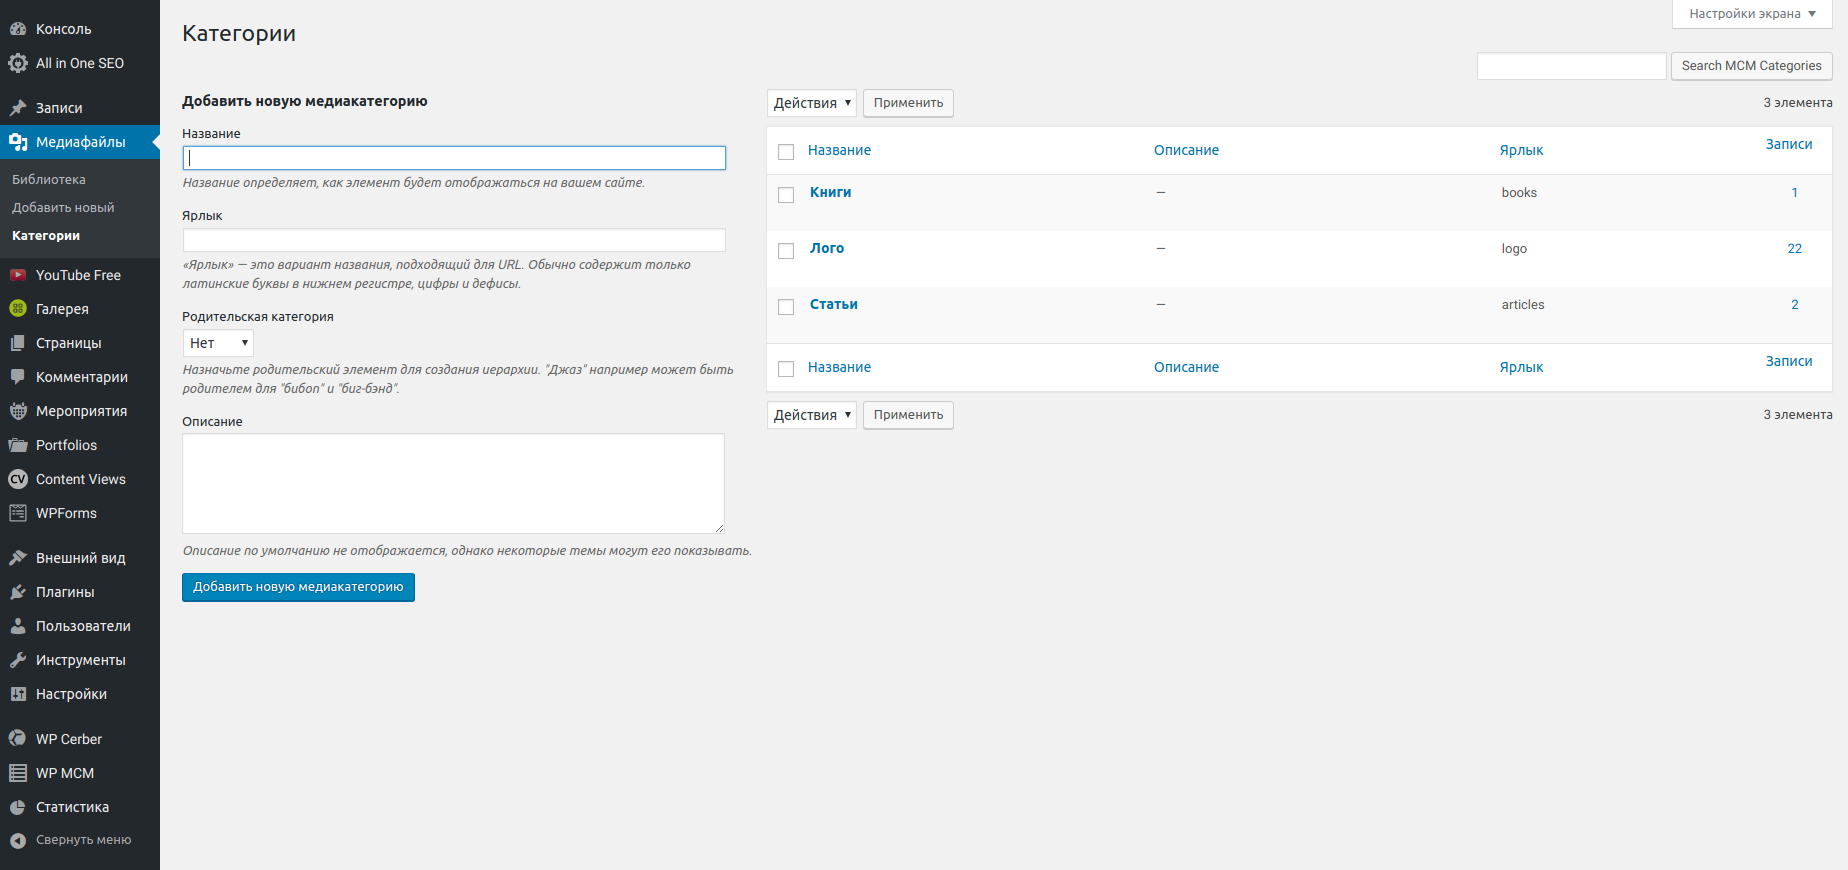
\includegraphics[width=\textwidth]{media_cat.png}
    \caption{Категории медиафайлов}
    \label{fig:pic_media_cat}
\end{figure}

\section{Загрузка медиафайлов}
\label{sec:part_upload}

На административной панели перейдите в меню «Медиафайлы/Добавить новый».
Появится страница, с которой вы можете «Загрузить новый медиафайл» или медиафайлы (см. рис. \ref{fig:pic_media_upload}).

\begin{figure}[htp]
    \centering
	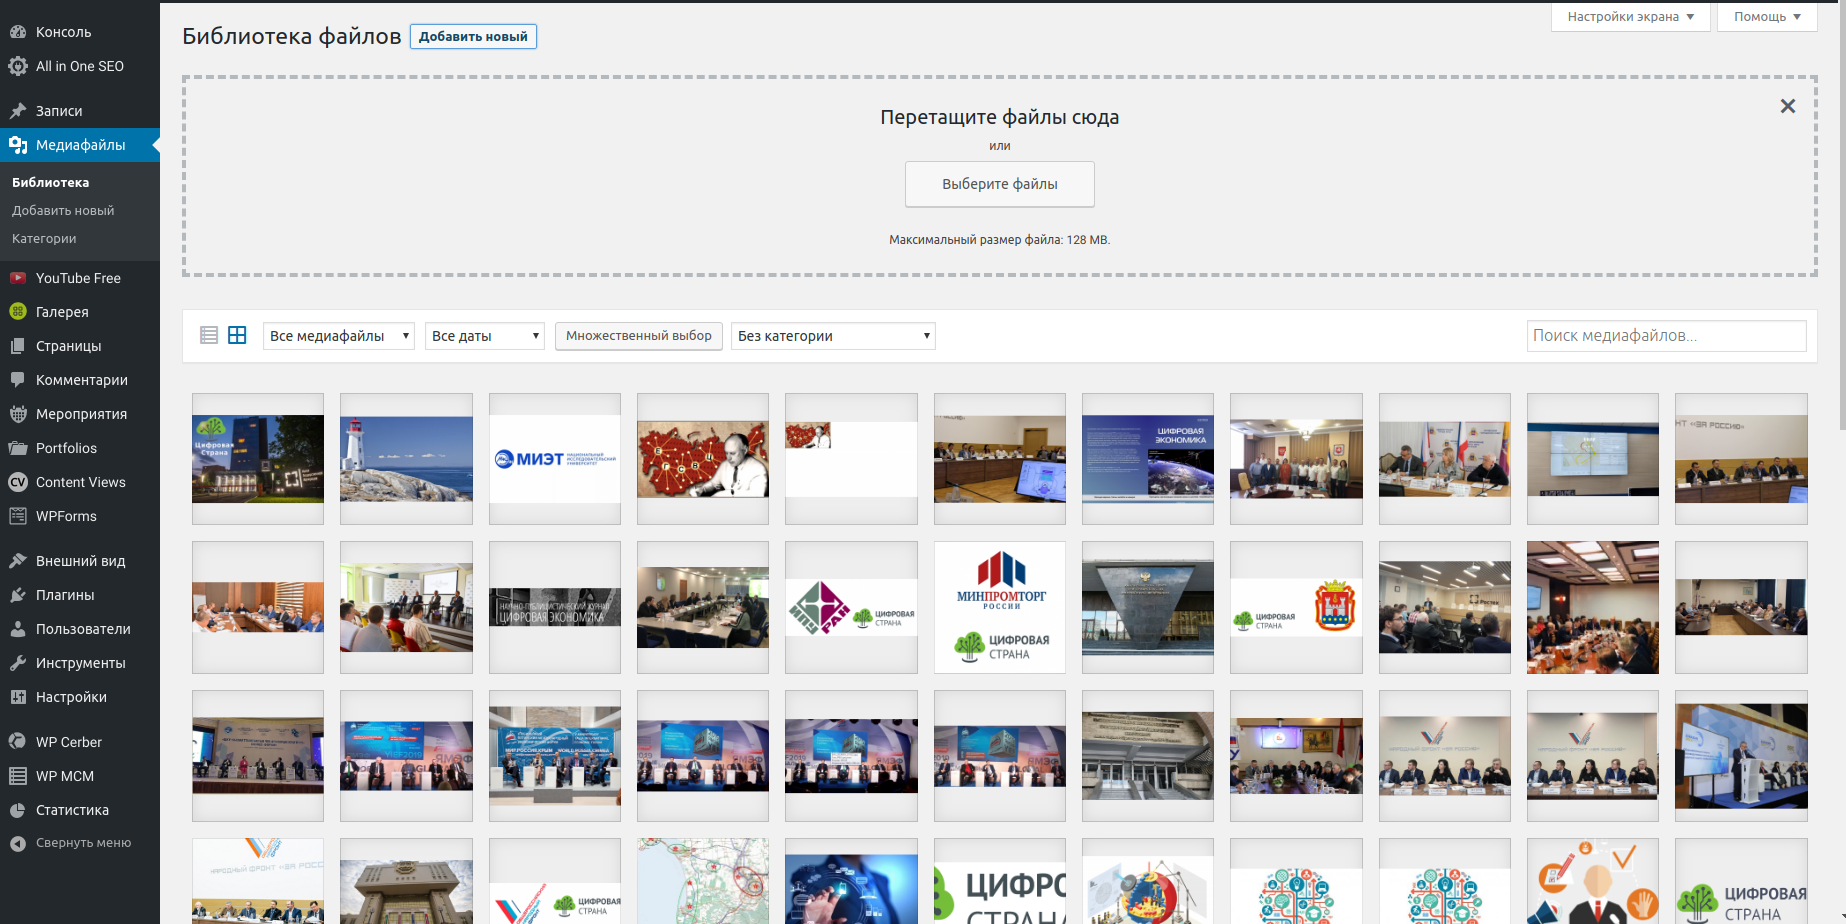
\includegraphics[width=\textwidth]{media_upload.png}
    \caption{Загрузка медиафайлов}
    \label{fig:pic_media_upload}
\end{figure}

После загрузки медиафайлов перейдите в меню «Медифайлы/Библиотека» и в раскрывающемся списке категорий выберите пункт «Без категории» (см. рис. \ref{fig:pic_media_no_cat}). Далее выберите медиафайл, появиться раздел «Media Categories» (Категории медиафайлов). Выберите категорию медиафайла.

\begin{figure}[htp]
    \centering
	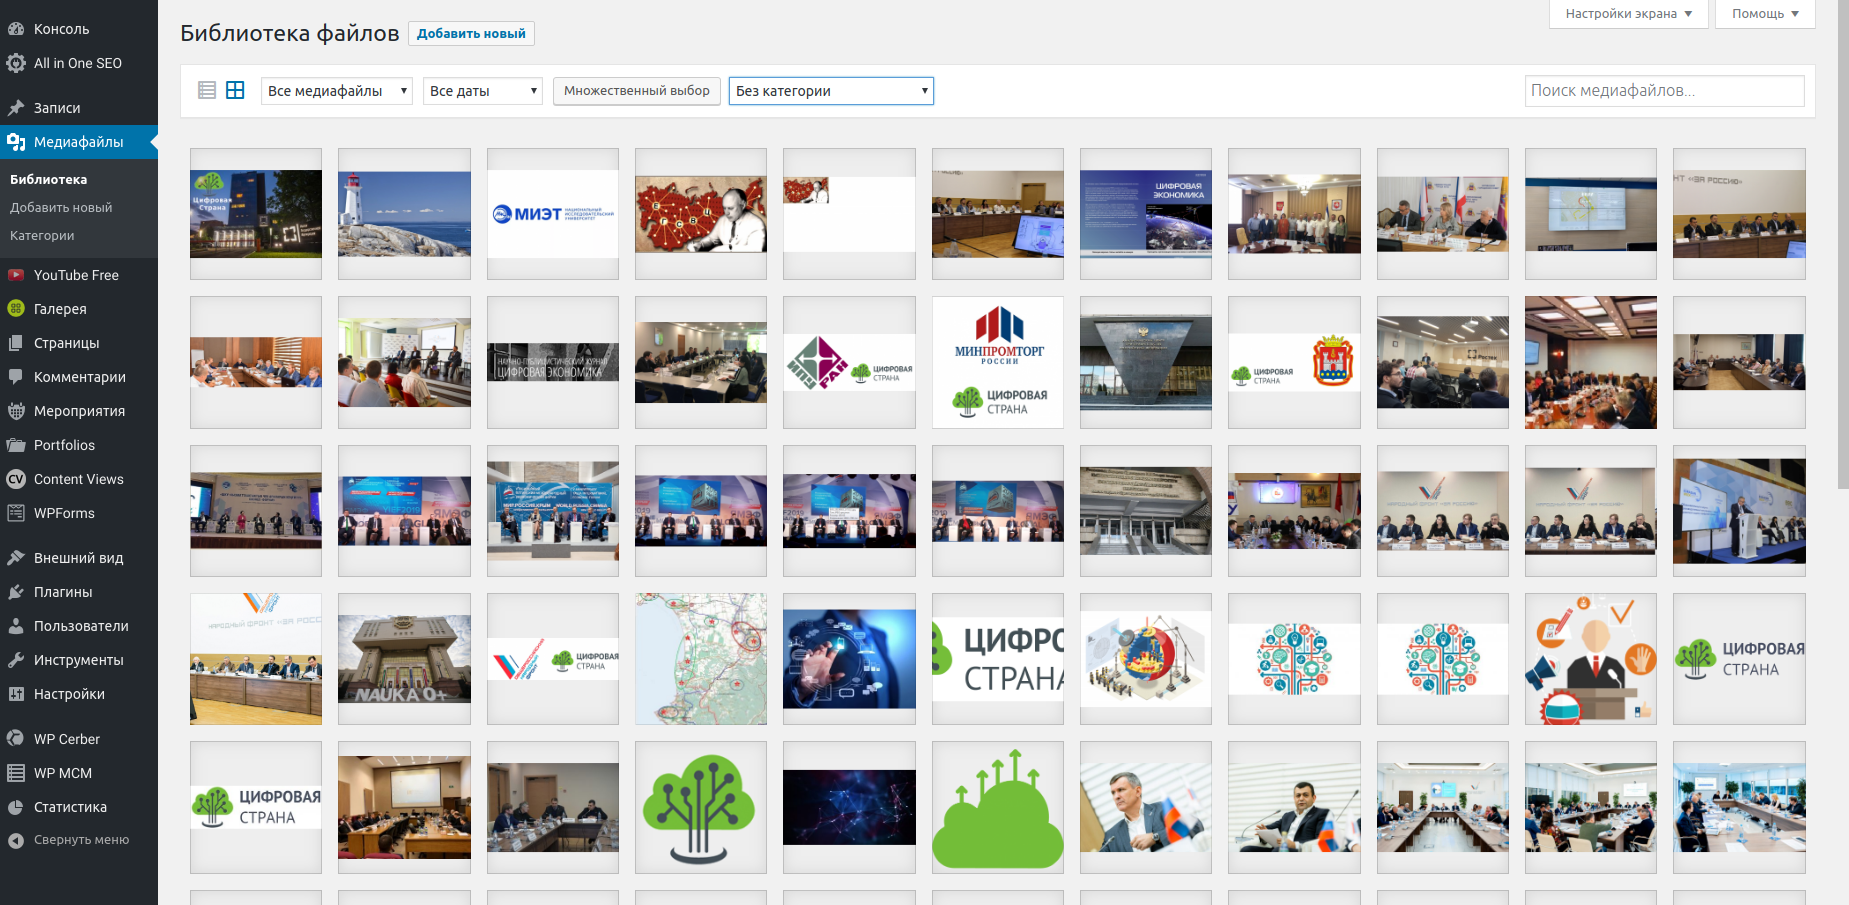
\includegraphics[width=\textwidth]{media_no_cat.png}
    \caption{Привязка медиафайла к категории}
    \label{fig:pic_media_no_cat}
\end{figure}

% 
\chapter{Страницы}
\label{sec:chapter_pages}

% 
\chapter{Записи}
\label{sec:chapter_posts}

\textbf{Записи} (или как их ещё называют — посты) — тип данных, который представляет собой привязанные к дате публикации, отсортированные в обратном хронологическом порядке материалы (новые — сверху, остальные выводятся на следующих страницах).
Записи используются для регулярных публикаций новостей, инструкций, статей, обзоров, отчётов. Список всех записей доступен в меню "Записи / Все записи" (см. рис. \ref{fig:pic_posts}).

\begin{figure}[htp]
    \centering
	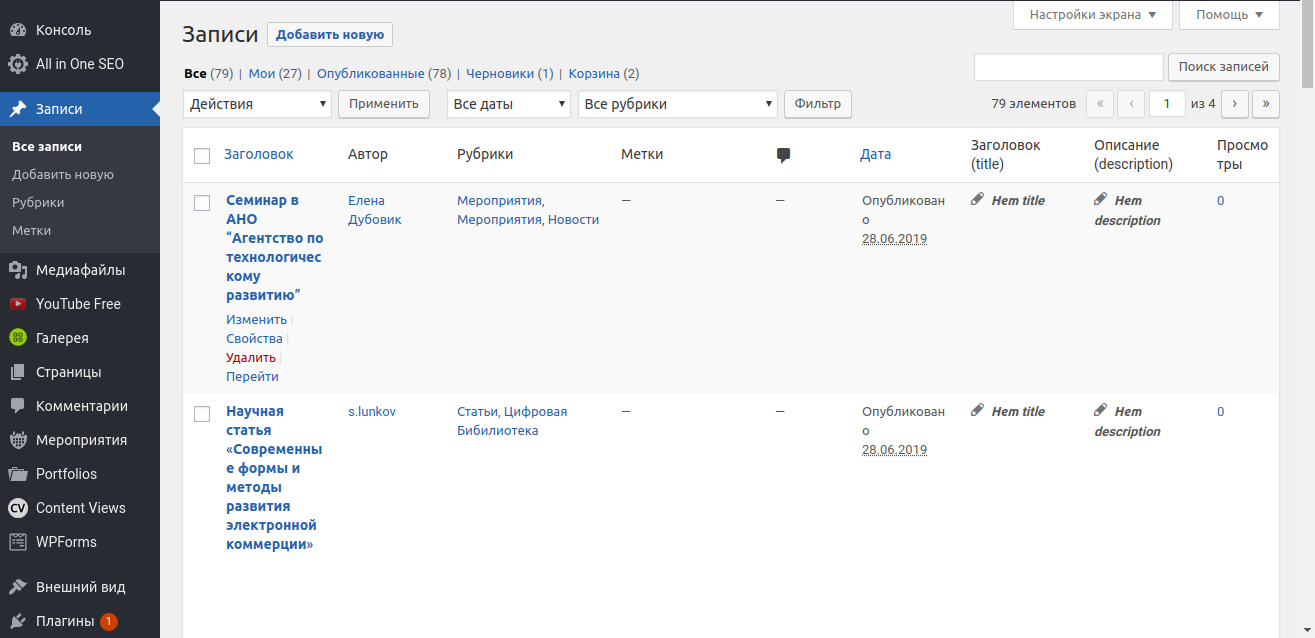
\includegraphics[width=\textwidth]{posts.png}
    \caption{Перечень записей}
    \label{fig:pic_posts}
\end{figure}

\section{Рубрики}
\label{sec:part_cat_posts}

Рубрики дают хорошую возможность группировать связанные записи, а также сообщить читателю, о чём запись. Рубрики также облегчают поиск материалов внутри вашего сайта. Рубрики могут иметь иерархическую структуру, для этого при создании дочерней рубрики установите необходимое значение в поле "Родительская рубрика".
Все записи могут относиться к одной или нескольким рубрикам. Для редактирования рубрик перейдите в меню «Записи / Рубрики» (см. рис. \ref{fig:pic_posts_cat})

\begin{figure}[htp]
    \centering
	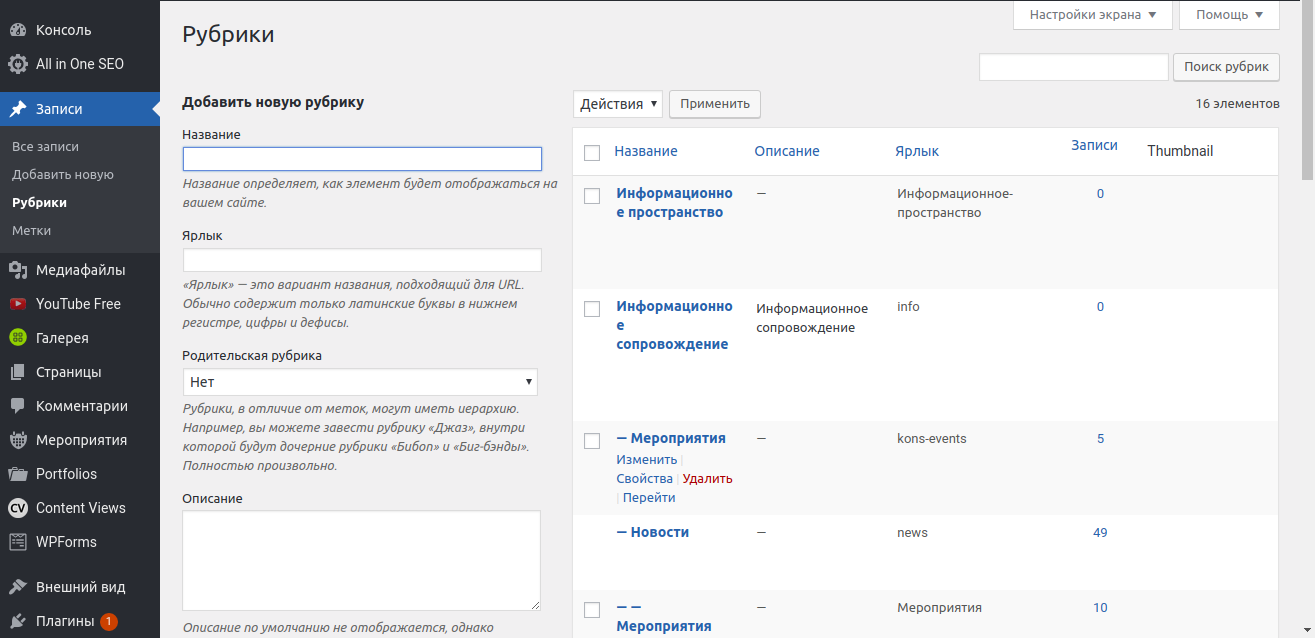
\includegraphics[width=\textwidth]{posts_cat.png}
    \caption{Рубрики»}
    \label{fig:pic_posts_cat}
\end{figure}


\section{Создание новой записи}
\label{sec:part_new_post}

Для публикации изображения к новости, перейдите в низ страницы раздел «Изображение записи» (см. рис. ниже)




Выберите изображение из медиа-библиотеки (см. рис. ниже)




После установки изображения нажмите кнопку «Опубликовать» (вверху страницы).


Нажмите кнопку «Добавить слайд» и в появившемся окне выберите изображение (см. рис. ниже)


Для каждого изображения в слайдере можно добавить описание. Для сохранения изменений в слайдере нажмите кнопку «Сохранить»

% 
\chapter{Слайдер}
\label{sec:chapter_slider}
% 
\chapter{События}
\label{sec:chapter_events}

Раздел «События» - элемент, в котором можно создавать и управлять своими событиями, изменять свои настройки.

Основные пункты меню:
\begin{itemize}
\item События - экран администратора для ваших событий.
\item Добавить событие - используйте для добавления нового события.
\item Event Tag - управляйте своими тегами событий. Используйте теги для организации ваших мероприятий.
\item Категории событий - управляйте категориями событий. Используйте категории для организации и классификации ваших событий.
\item Места - добавьте места и карты, которые можно прикрепить к вашим событиям.
\item Повторяющиеся события - используйте для создания повторяющихся событий.
\item Бронирование - управляйте своими заказами. Если вы являетесь профессиональным пользователем, вы также сможете управлять своими транзакциями.
\item Настройки - все настройки, необходимые для управления плагином Events Manager (см. п. \ref{sec:plugin_events_manager}).
\item Справка - найти ссылки на справку и список связанных с событием заполнителей, которые можно использовать для настройки событий.
\end{itemize}
% 
\chapter{Форум bbPress}
\label{sec:chapter_forum}

\textbf{Доски объявлений и форумы} – надежные инструменты, позволяющие создать онлайн-сообщества.

\section{Создание форума}
\label{sec:part_create_forum}

После установки bbPress добавит меню Форумы, Темы и Ответы в панель администратора WordPress.

Щелкаем по Форумы – Новый форум. Вы увидите экран, напоминающий область редактирования записей. Введите заголовок для вашего форума, а также его описание. После чего щелкните по кнопке Опубликовать.



\section{Вывод bbPress форума в фронтэнде WordPress}
\label{sec:part_forum_page}


Теперь, когда у вас есть несколько форумов, вы можете вывести на экран эти форумы во фронтэнде вашего сайта. Создайте новую страницу WordPress. Назовите ее как-нибудь, к примеру, Форум, Поддержка, Сообщество и т.д. Вставьте следующий шорткод на страницу:

\small
\begin{lstlisting}[frame=single, breaklines=true]
[ bbp-forum-index ]
\end{lstlisting}
\normalsize


Отключите комментарии и обратные ссылки для страницы, после чего опубликуйте ее.

Перейдите в раздел Внешний вид – Меню и добавьте эту страницу в навигационное меню.

Теперь, когда пользователь перейдет на эту страницу, он увидит полноценный форум.

\section{Пользовательские роли в bbPress}
\label{sec:part_forum_users}

bbPress идет вместе с предустановленными ролями, каждая со своими возможностями.

\begin{itemize}
\item Keymaster. Владелец сайта или администратор WordPress автоматически связывается с ролью Keymaster при установке bbPress. Keymaster может удалять и создавать форумы, создавать, редактировать, удалять все записи, темы, форумы.
\item Модераторы. Пользователи с ролью модератора имеют доступ к инструментам модерации, которые используются для управления форумами, темами и записями.
\item Участники. Стандартная пользовательская роль, участники могут создавать и редактировать свои собственные темы и ответы, могут добавлять темы в избранное и подписываться на темы.
\item Гости. Гости могут только читать форумы, темы и записи.
\item Заблокированные. Когда пользователь блокируется, все его возможности тоже блокируются. Такие пользователи могут читать публично доступные темы и ответы, но они не могут участвовать в обсуждении форума.
\end{itemize}% 
\chapter{Приложение}
\label{appendix:appendix}

\section{Плагины WordPress}
\label{sec:wp_plugins}

Для расширения функций WordPress используются плагины представленные ниже.
 
\subsection{Плагин Display Posts}
\label{sec:plugin_displayposts}

Плагин для отображения списка записей по категориям.

Адрес сайта: \url{https://displayposts.com/}

Руководство пользователя: \url{https://displayposts.com/docs/parameters/}

Пример настройки:
\small
\begin{lstlisting}[frame=single, breaklines=true]
[display-posts category_id="103" include_title="true" include_link="true" include_content="false" content_class="entry-content" order="ASC" include_excerpt_dash="true" excerpt_more="..." orderby="title" posts_per_page="1000"] 
\end{lstlisting}
\normalsize


\subsection{Плагин HTTP / HTTPS Remover}
\label{sec:plugin_http_https_remover}

Этот плагин создает относительные ссылки путем удаления http + https из URL.

Адрес сайта: \url{https://ru.wordpress.org/plugins/http-https-remover/}

\subsection{Плагин WP Statistics}
\label{sec:plugin_wp_statistics}

Полная аналитика и статистика для сайта на WordPress.

Адрес сайта: \url{https://ru.wordpress.org/plugins/wp-statistics/}

\subsection{Плагин PDF Embedder}
\label{sec:plugin_pdf_embedder}

Встраивайте PDF-файлы прямо в ваши записи и страницы, с гибкой шириной и высотой.

Адрес сайта: \url{https://ru.wordpress.org/plugins/pdf-embedder/}
Руководство пользователя: \url{https://wp-pdf.com/free-instructions/}

Пример настройки:
\small
\begin{lstlisting}[frame=single, breaklines=true]
[pdf-embedder url="https://mysite.com/wp-content/uploads/2015/01/Plan-Summary.pdf" width="500"]
\end{lstlisting}
\normalsize

\subsection{Плагин WP Media Category Management}
\label{sec:plugin_wp_media_category_management}

Плагин для обеспечения возможностей управления категориями медиафайлов в административном интерфейсе WordPress.

Адрес сайта: \url{http://ru.wordpress.org/plugins/wp-media-category-management/}

\subsection{Плагин Hide Featured Image}
\label{sec:plugin_hide_featured_image}

Плагин для отображения/скрытия избранных изображений на отдельных записях. Например избранные изображения отображаются, когда записи отображаются списком, но при входе в отдельную запись, избранное изображение не показывается.

Адрес сайта: \url{http://ru.wordpress.org/plugins/hide-featured-image/}

\subsection{Плагин Events Manager}
\label{sec:plugin_events_manager}

Плагин для регистрации событий и управление бронированием для WordPress. Позволяет создавать периодические события, указывать местоположения, использовать карты Google, RSS, поддерживает регистрацию бронирования и многое другое.

Адрес сайта: \url{http://ru.wordpress.org/plugins/events-manager/}

\subsection{Плагин Cerber Security, Antispam and Malware Scan}
\label{sec:plugin_serber}

Защищает WordPress от хакерских атак, спама, троянов и вредоносного ПО.
Предотвращает атаки перебора ограничением попыток входа через форму логина, XML-RPC/REST API и с использованием куки.
Отслеживает активность как пользователей так и нарушителей с уведомлениями по email, а также в браузере и на мобильных устройствах.
Защита от спама как собственными средствами, так и через. Google reCAPTCHA, для форм регистрации, форм контактов и комментариев.
Сканер на вредоносное ПО, проверка целостности и наблюдение за изменением файлов.
Усиление защиты WordPress гибкими правилами защиты и умными алгоритмами.
Ограничение доступа посредством черных и белых списков IP адресов.

Адрес сайта: \url{http://ru.wordpress.org/plugins/wp-cerber/}

\subsection{Плагин bbPress}
\label{sec:plugin_bbPress}

bbPress — простое и бесконечно мощное программное обеспечение для форума, созданное участниками разработки WordPress.
Форум bbPress прост в интеграции, лёгок в использовании и создан для масштабирования вместе с растущим сообществом.

Адрес сайта: \url{http://ru.wordpress.org/plugins/bbpress/}

\subsection{Плагин WP Super Cache}
\label{sec:plugin_wp_super_cache}

WP Super Cache самый популярный плагин для кеширования страниц в WordPress.
Плагин создаёт статичные html и php файлы – копии страниц WordPress и сохраняет их в кеш: /wp-content/cache/supercache/. Потом, при заходе пользователя на какую-либо страницу сайта, WordPress, вместо того, чтобы создать страницу с нуля, отдаёт браузеру заранее сохранённую копию html-страницы из кеша или собирает её максимально быстро из готовых php-файлов.

Адрес сайта: \url{http://ru.wordpress.org/plugins/wp-super-cache/}

\subsection{Плагин Yandex Mail}
\label{sec:plugin_yandex_mail}

Отправка писем через Yandex SMTP.

Адрес сайта: \url{http://ru.wordpress.org/plugins/yandex-mail/}

\subsection{Плагин Embed Plus for YouTube}
\label{sec:plugin_youtube}

Просмотр видео Youtube с сайта WordPress.

Адрес сайта: \url{http://ru.wordpress.org/plugins/youtube-embed-plus/}

\subsection{Плагин NextGEN Галерея}
\label{sec:plugin_NextGEN}

NextGEN Gallery — самый популярный плагин фотогалереи для WordPress, и, учитывая более 6 миллионов загрузок, это один из самых популярных WordPress плагинов в принципе. NextGEN позволяет вам создавать красивые галереи, у него много возможностей: загрузка больших изображений, группировка галерей в альбомы и многое другое.

Адрес сайта: \url{http://ru.wordpress.org/plugins/nextgen-gallery/}% 
\end{document}